%% EE568 HW2 -- Winding Design & Analysis Report
%% Compile: pdflatex EE568_HW2_Report_Sefer_IDACI_2575421.tex  (run twice)

\documentclass[12pt,a4paper]{article}

\usepackage[margin=2.5cm]{geometry}
\usepackage{amsmath, amssymb}
\usepackage{graphicx}
\usepackage{subcaption}
\usepackage{float}
\usepackage{hyperref}
\usepackage{enumitem}
\usepackage{booktabs}
\usepackage{array}
\usepackage{multirow}
\usepackage{fancyhdr}
\usepackage[table]{xcolor}
\usepackage[T1]{fontenc}
\usepackage[utf8]{inputenc}

\setlength{\headheight}{15pt}
\setlength{\parskip}{6pt}

\newcommand{\unit}[1]{\ensuremath{\,\mathrm{#1}}}
\newcommand{\degree}{\ensuremath{^{\circ}}}

\pagestyle{fancy}
\fancyhf{}
\lhead{EE568 -- Project 2}
\rhead{Sefer \.{I}DACI -- 2575421}
\rfoot{\thepage}

\hypersetup{colorlinks=true, linkcolor=blue!70!black}

% ============================================================
\begin{document}

% ---- Title Page -----------------------------------------------
\begin{titlepage}
  \centering
  \vspace*{3cm}
  {\Large Middle East Technical University \par}
  \vspace{0.4cm}
  {\large Department of Electrical and Electronics Engineering \par}
  \vspace{3cm}
  \rule{\linewidth}{0.5pt}\\[0.5cm]
  {\LARGE\bfseries EE568 -- Design of Electrical Machines \par}
  \vspace{0.4cm}
  {\large\bfseries Project 2: Motor Winding Design \& Analysis \par}
  \rule{\linewidth}{0.5pt}\\[2cm]
  \begin{tabular}{ll}
    \textbf{Name:}           & Sefer \.{I}DACI \\[6pt]
    \textbf{Student Number:} & 2575421          \\[6pt]
    \textbf{Design:}         & Design 1 -- $N_s=15$, $N_m=8$ \\[6pt]
    \textbf{Date:}           & June 2026        \\
  \end{tabular}
  \vfill
  {\small Submitted to: EE568 Course Staff}
\end{titlepage}

\tableofcontents
\newpage

% ============================================================
\section{Introduction}

This report presents the winding design and analytical modelling of a
three-phase surface-mount permanent-magnet synchronous machine (SPMSM).
The assigned design is \textbf{Design~1} (student ID~2575421,
$2575421 \bmod 5 = 1$), with $N_s = 15$ stator slots and $N_m = 8$
rotor poles ($p = 4$ pole-pairs).

The report is organised as follows.
Section~\ref{sec:theory} provides the theoretical background from standard
references.
Section~\ref{sec:q1} covers integral-slot winding design for a 72-slot,
6-pole machine.
Section~\ref{sec:q2} presents the fractional-slot winding analysis for
Design~1.
Section~\ref{sec:q3} contains all analytical modelling calculations.
Section~\ref{sec:q4} will present the 2D FEA results from ANSYS Maxwell.

% ============================================================
\section{Theoretical Background}
\label{sec:theory}

\subsection{Winding Fundamentals}

An AC machine winding converts an applied current distribution into a
rotating magnetomotive force (MMF) and, in the generating case, converts
a rotating flux into an induced electromotive force (EMF).
The quality of this conversion is quantified by the \emph{winding factor}
$k_w$, which accounts for the spatial distribution of conductors
\cite{Pyrhonen2014,Hanselman2006}.

\subsubsection{MMF Distribution and Harmonics}

For a coil placed in slots the MMF is not sinusoidal but contains
space harmonics whose order is $n = 1, 5, 7, 11, \ldots$
(for a balanced three-phase winding with no triplen harmonics).
The $n$-th space harmonic amplitude is reduced relative to the
fundamental by the \emph{harmonic winding factor} $k_{w,n}$ \cite{Pyrhonen2014}.

Suppressing high-order space harmonics is desirable because they
increase iron losses, create parasitic torque pulsations, and generate
acoustic noise.

\subsection{Integral-Slot Distributed Winding}

An integral-slot winding has an integer number of slots per pole per phase:
\begin{equation}
  q = \frac{N_s}{2p \, m} \in \mathbb{Z}^+
\end{equation}
For the 72-slot, 6-pole, three-phase machine of Q1: $q = 72/(6\times3) = 4$.

\subsubsection{Distribution Factor}

When $q$ coils are placed in adjacent slots separated by one slot pitch
$\alpha_e$ (electrical), their phasors are offset and the resultant EMF
is smaller than the arithmetic sum.
The ratio is the distribution factor \cite[Ch.\,4]{Pyrhonen2014}:
\begin{equation}
  k_{d,n} = \frac{\sin\!\bigl(n\,q\,\alpha_e/2\bigr)}
                 {q\,\sin\!\bigl(n\,\alpha_e/2\bigr)},
  \qquad
  \alpha_e = \frac{p \cdot 360\degree}{N_s}
  \label{eq:kd}
\end{equation}
For the fundamental ($n=1$) a larger $q$ brings $k_{d,1}$ closer to unity
and simultaneously reduces higher harmonics.

\subsubsection{Pitch Factor}

A full-pitched coil has its sides exactly one pole pitch $\tau_p$ apart.
Shortening the coil to $y < \tau_p$ introduces a phase shift between the
two sides, yielding the pitch factor \cite[Ch.\,4]{Pyrhonen2014}:
\begin{equation}
  k_{p,n} = \sin\!\left(\frac{n\,y\,\pi}{2\,\tau_p}\right)
  \label{eq:kp}
\end{equation}
Short-pitching by $1/n$ of the pole pitch eliminates the $n$-th harmonic
entirely ($k_{p,n}=0$).
The 11/12 short pitch ($y = 11$, $\tau_p = 12$) is chosen to suppress
the 11th and 13th harmonics in a three-phase machine \cite{Chapman2012}.

\subsubsection{Winding Factor}

The overall winding factor is:
\begin{equation}
  k_{w,n} = k_{d,n} \cdot k_{p,n}
  \label{eq:kw}
\end{equation}
A high $k_{w,1}$ maximises torque density; a low $k_{w,n}$ for $n > 1$
reduces harmonic content.

\subsection{Fractional-Slot Concentrated Winding (FSCW)}

In a fractional-slot winding $q \notin \mathbb{Z}^+$, meaning the number
of slots per pole is not an integer.
When $q < 1$ and each coil is wound around a single tooth (coil pitch = 1
slot), the winding is called a \emph{concentrated} or \emph{tooth-coil}
winding.
This topology offers short end-windings, high slot fill factors, and
easy manufacture, at the cost of lower fundamental winding factor and
richer harmonic spectrum compared to a distributed winding
\cite[Ch.\,4]{Hanselman2006}.

\subsubsection{Star-of-Slots Method}

For a fractional-slot winding the winding factor cannot be computed from
simple closed-form expressions; instead the \emph{star of slots} (phasor
diagram) method is used \cite{Pyrhonen2014,Meier2008}.

Each slot $k$ is assigned an EMF phasor at electrical angle:
\begin{equation}
  \varphi_k = (k-1)\,\alpha_s \pmod{360\degree},
  \qquad
  \alpha_s = \frac{N_m \cdot 180\degree}{N_s}
  \label{eq:phi_k}
\end{equation}
The $N_s$ phasors form the \emph{star of slots}.
For a three-phase winding the circle is divided into six $60\degree$
sectors and each phasor is assigned to the phase whose axis is nearest:
\begin{center}
  A$+$: $[0\degree, 60\degree)$;\quad
  C$-$: $[60\degree, 120\degree)$;\quad
  B$+$: $[120\degree, 180\degree)$;\quad
  A$-$: $[180\degree, 240\degree)$;\quad
  C$+$: $[240\degree, 300\degree)$;\quad
  B$-$: $[300\degree, 360\degree)$
\end{center}

The $n$-th harmonic winding factor is then \cite{Pyrhonen2014}:
\begin{equation}
  k_{w,n} = \frac{1}{N_{ph}}
  \left|\sum_{k \in \text{ph}^+} e^{j\,n\varphi_k}
        + \sum_{k \in \text{ph}^-} e^{j(n\varphi_k + \pi)}\right|
  \label{eq:kw_fscw}
\end{equation}
where $N_{ph}$ is the number of slots per phase, and
$\text{ph}^+$, $\text{ph}^-$ are the positive and negative slot sets
of that phase.

\subsection{Analytical Machine Modelling}

\subsubsection{Air-Gap Flux Density -- Surface PM Machine}

For a surface-mount PM machine with radially magnetised magnets, treating
the rotor surface and stator bore as concentric cylinders, the peak
air-gap flux density is \cite[Ch.\,3]{Hanselman2006}:
\begin{equation}
  B_{g,\text{peak}} = \frac{B_r \, l_m}{l_m + \mu_r \, k_c \, g}
  \label{eq:Bg}
\end{equation}
where $B_r$ is the remanence, $l_m$ the magnet radial thickness,
$\mu_r$ the magnet relative permeability, $g$ the physical air gap,
and $k_c$ Carter's coefficient.

\subsubsection{Carter's Coefficient}

Stator slotting increases the effective air gap.
Carter's coefficient accounts for this by replacing the slotted stator
with an equivalent smooth surface \cite{Carter1901,Pyrhonen2014}:
\begin{equation}
  k_c = \frac{\tau_s}{\tau_s - \gamma}, \qquad
  \gamma = \frac{4g}{\pi}\left[\frac{w_s}{2g}
           \arctan\!\frac{w_s}{2g}
           - \ln\!\sqrt{1+\!\left(\frac{w_s}{2g}\right)^{\!2}}\,\right]
  \label{eq:kc}
\end{equation}
where $\tau_s = 2\pi R_{si}/N_s$ is the slot pitch at the stator bore and
$w_s$ is the slot opening width.

\subsubsection{Effective Axial Length}

Fringing at the axial ends of the machine extends the effective flux-linking
length beyond the physical stack length $L_s$.
A common approximation is \cite[Ch.\,5]{Hanselman2006}:
\begin{equation}
  L_e = L_s + 2g
  \label{eq:Le}
\end{equation}

\subsubsection{Electrical Loading}

The linear current density (electrical loading) characterises the ampere-conductor
loading on the stator bore circumference \cite{Pyrhonen2014}:
\begin{equation}
  A_{rms} = \frac{J_{rms}\,k_{wc}\,A_{slot}}{\tau_s}
  \label{eq:Arms}
\end{equation}
where $J_{rms}$ is the rms current density in the conductors,
$k_{wc}$ the slot fill factor, and $A_{slot}$ the net slot cross-section.

\subsubsection{Electromagnetic Torque -- Shear Stress Approach}

The electromagnetic shear stress acting at the stator bore is
\cite[Ch.\,3]{Hanselman2006}:
\begin{equation}
  \sigma = \frac{1}{2}\,k_{w,1}\,B_{g,\text{peak}}\,A_{peak}
         = \frac{1}{\sqrt{2}}\,k_{w,1}\,B_{g,\text{peak}}\,A_{rms}
  \label{eq:sigma}
\end{equation}
The resulting average electromagnetic torque and shaft power are:
\begin{equation}
  T = \sigma \cdot 2\pi R_{si}^2 L_e,
  \qquad
  P = T\,\omega_m
  \label{eq:T}
\end{equation}

\subsubsection{Flux Per Pole}

The flux per pole, needed to size the back-iron and to calculate the
induced EMF, is \cite[Ch.\,2]{Hanselman2006}:
\begin{equation}
  \Phi_{pole} = B_{g,\text{peak}}\,\alpha_m\,\tau_p\,L_e,
  \qquad
  \tau_p = \frac{\pi R_{si}}{p}
  \label{eq:Phi}
\end{equation}
where $\alpha_m = \theta_m/180\degree$ is the magnet arc ratio
(160$\degree$/180$\degree$ = 0.889 here) and $\tau_p$ is the pole pitch
at the stator bore.

\subsubsection{Back-Iron Sizing}

The stator and rotor yoke widths are set so that the peak flux density
in the iron does not exceed the target $B_t = 1.4\unit{T}$
\cite[Ch.\,5]{Hanselman2006}:
\begin{equation}
  w_{sy} = \frac{\Phi_{pole}}{2\,B_t\,L_e},
  \qquad
  w_{ry} = \frac{\Phi_{pole}}{2\,B_t\,L_e}
  \label{eq:yoke}
\end{equation}

% ============================================================
\section{Q1 -- Integral-Slot Winding Design}
\label{sec:q1}

% ---- 1.1 -------------------------------------------------------
\subsection{Machine Parameters and Notation}

The given machine has the following specifications:

\begin{table}[H]
  \centering
  \caption{Given and derived parameters -- Q1}
  \label{tab:q1_params}
  \begin{tabular}{llcc}
    \toprule
    Parameter & Meaning & Symbol & Value \\
    \midrule
    Number of stator slots   & Total slots around the stator bore   & $N_s$      & 72 \\
    Number of poles          & Total magnetic poles on the rotor     & $2p$       & 6  \\
    Number of pole pairs     & Half the pole count; $p = 2p/2$       & $p$        & 3  \\
    Number of phases         & Phases of the AC supply               & $m$        & 3  \\
    Winding layers           & Number of coil sides per slot         & ---        & 2 (double-layer) \\
    \bottomrule
  \end{tabular}
\end{table}

\noindent\textbf{Notation used throughout:}
\begin{itemize}[noitemsep]
  \item $N_s$ -- total number of stator slots.
  \item $p$ -- number of pole pairs (a 6-pole machine has $p=3$).
  \item $m$ -- number of phases ($m=3$).
  \item $\alpha_e$ -- \emph{electrical angle per slot}: the angle (in electrical
        degrees) between the EMF phasors of two adjacent slots.
  \item $q$ -- \emph{slots per pole per phase}: how many consecutive slots are
        occupied by one phase under one pole.
  \item $\tau_p$ -- \emph{pole pitch} in slots: the number of slots spanned by one pole.
  \item $y$ -- \emph{coil pitch} (or coil span) in slots: the number of slots between
        the two sides of one coil.
  \item $k_d$, $k_p$, $k_w$ -- distribution, pitch, and winding factors, respectively.
  \item Superscript or subscript $n$ denotes the harmonic order ($n=1,3,5,\ldots$).
  \item A$+$/A$-$ means Phase~A current flows \emph{into} / \emph{out of} the page.
\end{itemize}

% ---- 1.2 -------------------------------------------------------
\subsection{Step 1 -- Derived Quantities}

\subsubsection{Electrical Angle per Slot $\alpha_e$}

The stator has $N_s = 72$ slots arranged uniformly around the bore.
One full revolution is $360\degree$ mechanical, but in electrical terms
the field repeats once per pole pair, so one full electrical cycle
corresponds to $360\degree/p$ mechanical degrees.
The electrical angle between two adjacent slots is therefore:
\begin{equation}
  \boxed{\alpha_e = \frac{p \times 360\degree}{N_s}}
  = \frac{3 \times 360\degree}{72} = \mathbf{15\degree\,\text{(electrical)}}
  \label{eq:alpha_e}
\end{equation}

\subsubsection{Slots per Pole per Phase $q$}

The total number of slots is shared equally among $2p$ poles and $m$ phases:
\begin{equation}
  \boxed{q = \frac{N_s}{2p \cdot m}}
  = \frac{72}{6 \times 3} = \mathbf{4}
  \label{eq:q}
\end{equation}
Because $q = 4 \in \mathbb{Z}^+$, this is an \emph{integral-slot} winding.
Each phase occupies 4 consecutive slots under each pole.

\subsubsection{Pole Pitch $\tau_p$}

The pole pitch is the number of slots under one pole:
\begin{equation}
  \boxed{\tau_p = \frac{N_s}{2p}}
  = \frac{72}{6} = \mathbf{12\,\text{slots}}
  \label{eq:tau_p}
\end{equation}
A \emph{full-pitched} coil spans exactly $\tau_p = 12$ slots.

\subsubsection{One Pole-Pair $= 360\degree$ electrical $= 24$ slots}

Since $\alpha_e = 15\degree$, it takes $360\degree / 15\degree = 24$ slots
to complete one full electrical cycle.
This means \textbf{one pole-pair spans 24 consecutive slots}, which is the
minimum repeating unit of the winding.

% ---- 1.3 -------------------------------------------------------
\subsection{Step 2 -- Upper Layer Assignment (the $60\degree$ Sector Rule)}

\subsubsection{Physical Basis}

Each stator slot has a conductor whose induced EMF is represented by a phasor.
The phasor of slot $k$ (upper layer) points at electrical angle:
\begin{equation}
  \varphi_k = (k-1)\,\alpha_e \pmod{360\degree}
  \label{eq:slot_angle}
\end{equation}

For a balanced 3-phase winding the $360\degree$ circle is divided into
\textbf{six sectors of $60\degree$} each, alternating between positive and
negative directions of the three phases.
The sector assignment follows the positive phase sequence A$\to$B$\to$C:

\begin{center}
\begin{tabular}{ccc}
  \toprule
  Sector & Angle range & Assignment \\
  \midrule
  1 & $[0\degree,\;60\degree)$   & A$+$ \\
  2 & $[60\degree,\;120\degree)$ & C$-$ \\
  3 & $[120\degree,\;180\degree)$& B$+$ \\
  4 & $[180\degree,\;240\degree)$& A$-$ \\
  5 & $[240\degree,\;300\degree)$& C$+$ \\
  6 & $[300\degree,\;360\degree)$& B$-$ \\
  \bottomrule
\end{tabular}
\end{center}

\noindent Why this ordering?
Phase A peaks at $0\degree$.
Between A's peak ($0\degree$) and B's peak ($120\degree$), the phase that
is most negative is C (it is at $-60\degree$ relative to its own peak),
so the sector $[60\degree,120\degree)$ is labelled C$-$.
Between B's peak and C's peak the lagging phase A is most negative, hence
A$-$ at $[180\degree,240\degree)$, and so on.
The result is a sequence that exactly places 4 slots (one group of $q=4$) in
each sector because $4 \times 15\degree = 60\degree$ fills one sector
precisely.

\subsubsection{Slot Angle Table -- One Pole-Pair (Slots 1--24)}

\begin{table}[H]
  \centering
  \caption{Upper-layer phase assignment for one pole-pair (72-slot, 6-pole)}
  \label{tab:q1_upper}
  \begin{tabular}{ccccc|ccccc}
    \toprule
    Slot $k$ & $\varphi_k$ & Sector & Layer-1 &&
    Slot $k$ & $\varphi_k$ & Sector & Layer-1 \\
    \midrule
    1  & $0\degree$   & 1 & A$+$ && 13 & $180\degree$ & 4 & A$-$ \\
    2  & $15\degree$  & 1 & A$+$ && 14 & $195\degree$ & 4 & A$-$ \\
    3  & $30\degree$  & 1 & A$+$ && 15 & $210\degree$ & 4 & A$-$ \\
    4  & $45\degree$  & 1 & A$+$ && 16 & $225\degree$ & 4 & A$-$ \\
    5  & $60\degree$  & 2 & C$-$ && 17 & $240\degree$ & 5 & C$+$ \\
    6  & $75\degree$  & 2 & C$-$ && 18 & $255\degree$ & 5 & C$+$ \\
    7  & $90\degree$  & 2 & C$-$ && 19 & $270\degree$ & 5 & C$+$ \\
    8  & $105\degree$ & 2 & C$-$ && 20 & $285\degree$ & 5 & C$+$ \\
    9  & $120\degree$ & 3 & B$+$ && 21 & $300\degree$ & 6 & B$-$ \\
    10 & $135\degree$ & 3 & B$+$ && 22 & $315\degree$ & 6 & B$-$ \\
    11 & $150\degree$ & 3 & B$+$ && 23 & $330\degree$ & 6 & B$-$ \\
    12 & $165\degree$ & 3 & B$+$ && 24 & $345\degree$ & 6 & B$-$ \\
    \midrule
    \multicolumn{4}{c}{\textbf{Pole 1} (0\degree--165\degree)} &&
    \multicolumn{4}{c}{\textbf{Pole 2} (180\degree--345\degree)} \\
    \bottomrule
  \end{tabular}
\end{table}

\noindent Note how Pole~2 (slots 13--24) is the \emph{sign-flipped mirror} of Pole~1:
A$+\to$A$-$, C$-\to$C$+$, B$+\to$B$-$.
This is automatic: each slot in Pole~2 is exactly $12 \times 15\degree = 180\degree$
ahead of the corresponding slot in Pole~1, placing it in the opposite sector.
This $180\degree$ phase reversal is what makes the two poles magnetically opposite
(one North, one South).

% ---- 1.4 -------------------------------------------------------
\subsection{Step 3 -- Lower Layer Assignment}

\subsubsection{The Coil Concept}

A double-layer winding fills each slot with \emph{two} coil sides: Layer~1
(upper) and Layer~2 (lower).
One coil consists of a \textbf{go side} in the upper layer of slot $k$ and a
\textbf{return side} in the lower layer of slot $k+y$, where $y$ is the coil
pitch (Figure~\ref{fig:coil_concept}).

\begin{figure}[H]
\centering
\begin{tabular}{ccccc}
  Slot $k$ & & & & Slot $k+y$ \\
  \framebox[1.5cm]{$\bullet$ (up)} & $\xrightarrow{\text{coil}}$ & & $\xrightarrow{}$ &
  \framebox[1.5cm]{$\times$ (lo)} \\
  go side & & & & return side \\
  current in & & & & current out \\
\end{tabular}
\caption{One coil: go side (upper layer, slot $k$) and return side (lower layer, slot $k+y$).}
\label{fig:coil_concept}
\end{figure}

Therefore, reading it from the perspective of the \emph{lower layer of slot $j$}:
\begin{equation}
  \text{Layer-2 of slot }j
  = \text{opposite direction of Layer-1 of slot }(j - y)
  \label{eq:lower_rule}
\end{equation}
``Opposite direction'' means: if Layer-1 of slot $j-y$ is A$+$ (current in),
then Layer-2 of slot $j$ is A$-$ (current out), and vice versa.

\subsubsection{Full-Pitched Winding ($y = 12$)}

Apply rule~\eqref{eq:lower_rule} with $y=12$.
Three representative slots are shown; all 24 follow the same logic:

\begin{center}
\begin{tabular}{cccc}
  \toprule
  Slot $j$ & Layer-1 of slot $j-12$ & $\Rightarrow$ Layer-2 of slot $j$ \\
  \midrule
  1  & Layer-1[13] $=$ A$-$ & A$+$ \\
  5  & Layer-1[17] $=$ C$+$ & C$-$ \\
  13 & Layer-1[1]  $=$ A$+$ & A$-$ \\
  \bottomrule
\end{tabular}
\end{center}

\noindent\textbf{Key geometric reason:}
The electrical angle difference between slot $j$ and slot $j-12$ is
$12 \times 15\degree = 180\degree$ exactly.
Every slot is therefore opposite (in phasor sense) to its partner 12 slots away.
Flipping the direction cancels the sign: $-(\text{A}-) = \text{A}+$.
As a result, \textbf{both layers in every slot carry the same phase in the same direction}:

\begin{center}
\small
\begin{tabular}{r|*{4}{c}|*{4}{c}|*{4}{c}|*{4}{c}|*{4}{c}|*{4}{c}}
  \toprule
  Slot: & 1&2&3&4 & 5&6&7&8 & 9&10&11&12 & 13&14&15&16 & 17&18&19&20 & 21&22&23&24\\
  \midrule
  Layer 1: & \multicolumn{4}{c|}{A$+$} & \multicolumn{4}{c|}{C$-$} & \multicolumn{4}{c|}{B$+$} &
             \multicolumn{4}{c|}{A$-$} & \multicolumn{4}{c|}{C$+$} & \multicolumn{4}{c}{B$-$}\\
  Layer 2: & \multicolumn{4}{c|}{A$+$} & \multicolumn{4}{c|}{C$-$} & \multicolumn{4}{c|}{B$+$} &
             \multicolumn{4}{c|}{A$-$} & \multicolumn{4}{c|}{C$+$} & \multicolumn{4}{c}{B$-$}\\
  \bottomrule
\end{tabular}
\end{center}

\noindent The coil pitch arrow: $\underbrace{1 \xrightarrow{\;y=12\;} 13}_{\text{Phase A coil 1}}$,
$\underbrace{2 \xrightarrow{} 14}_{\text{coil 2}}$, $\ldots$

\subsubsection{11/12 Short-Pitched Winding ($y = 11$)}

Now $y = 11$: the angle difference between slot $j$ and slot $j-11$ is
$11 \times 15\degree = 165\degree$ (not $180\degree$).
At group boundaries the phasor falls in the adjacent sector instead of the
opposite one, creating \emph{mixed-phase} slots.

\begin{center}
\small
\begin{tabular}{r|*{4}{c}|*{4}{c}|*{4}{c}|*{4}{c}|*{4}{c}|*{4}{c}}
  \toprule
  Slot: & 1&2&3&4 & 5&6&7&8 & 9&10&11&12 & 13&14&15&16 & 17&18&19&20 & 21&22&23&24\\
  \midrule
  Layer 1: & \multicolumn{4}{c|}{A$+$} & \multicolumn{4}{c|}{C$-$} & \multicolumn{4}{c|}{B$+$} &
             \multicolumn{4}{c|}{A$-$} & \multicolumn{4}{c|}{C$+$} & \multicolumn{4}{c}{B$-$}\\
  Layer 2: & A$+$&A$+$&A$+$&\cellcolor{yellow!50}C$-$ &
             C$-$&C$-$&C$-$&\cellcolor{yellow!50}B$+$ &
             B$+$&B$+$&B$+$&\cellcolor{yellow!50}A$-$ &
             A$-$&A$-$&A$-$&\cellcolor{yellow!50}C$+$ &
             C$+$&C$+$&C$+$&\cellcolor{yellow!50}B$-$ &
             B$-$&B$-$&B$-$&\cellcolor{yellow!50}A$+$ \\
  \bottomrule
\end{tabular}
\end{center}

\noindent The highlighted (yellow) slots (4, 8, 12, 16, 20, 24) are the \emph{boundary slots}
where two different phases share the same slot.
They arise because shortening the pitch by 1 slot shifts the return conductor
out of the purely opposite sector by $180\degree - 165\degree = 15\degree$
(one slot), crossing into the adjacent group.

\noindent Worked example for boundary slot $j=4$:
\begin{quote}
  Layer-1 of slot $j-11 = $ slot $-7 \equiv$ slot $17$ (wrap by adding 24)
  $=$ C$+$.\\
  Layer-2 of slot 4 $= -$(C$+$) $=$ C$-$.\\
  But Layer-1 of slot 4 $=$ A$+$. $\Rightarrow$ \textbf{mixed: A$+$/C$-$}.
\end{quote}

% ---- 1.5 -------------------------------------------------------
\subsection{Step 4 -- Distribution Factor $k_d$}

\subsubsection{Physical Meaning}

In a concentrated winding (all $q$ coils of one phase under one pole placed
in a single slot) the coil EMFs are perfectly in phase and add arithmetically.
In a \emph{distributed} winding the $q$ coils are spread over $q$ adjacent
slots, each displaced by $\alpha_e$ electrically.
Their EMF phasors form an arc of a regular polygon, and the vector sum is
smaller than the arithmetic sum.

\begin{equation}
  k_d = \frac{\text{vector (phasor) sum of the }q\text{ coil EMFs}}
             {\text{arithmetic sum of the }q\text{ coil EMFs}}
\end{equation}

\subsubsection{Derivation}

Each of the $q$ phasors has magnitude $E_m$ and successive phasors are
offset by $\alpha_e$.
The vector sum of $q$ unit phasors starting at $0\degree$ and stepping by $\alpha_e$:
\begin{equation}
  \left|\sum_{i=0}^{q-1} e^{j\,i\,\alpha_e}\right|
  = \frac{\sin(q\,\alpha_e/2)}{\sin(\alpha_e/2)}
\end{equation}
(standard result for a finite geometric series on the unit circle).
The arithmetic sum is simply $q$.
Hence:
\begin{equation}
  \boxed{k_{d,n} = \frac{\sin\!\left(\dfrac{n\,q\,\alpha_e}{2}\right)}
                        {q\,\sin\!\left(\dfrac{n\,\alpha_e}{2}\right)}}
  \label{eq:kd_q1}
\end{equation}
where $n$ is the harmonic order.
For the $n$-th harmonic the electrical angle between adjacent phasors becomes
$n\,\alpha_e$, so $\alpha_e$ is replaced by $n\,\alpha_e$ throughout.

\subsubsection{Calculations for $q=4$, $\alpha_e = 15\degree$}

\textbf{Fundamental ($n=1$):}
\begin{align}
  k_{d,1} &= \frac{\sin\!\left(\dfrac{1 \times 4 \times 15\degree}{2}\right)}
                  {4\,\sin\!\left(\dfrac{1 \times 15\degree}{2}\right)}
           = \frac{\sin 30\degree}{4\,\sin 7.5\degree}
           = \frac{0.5000}{4 \times 0.1305}
           = \frac{0.5000}{0.5221}
           = \mathbf{0.9577}
\end{align}

\textbf{Third harmonic ($n=3$):}
\begin{align}
  k_{d,3} &= \frac{\sin\!\left(\dfrac{3 \times 4 \times 15\degree}{2}\right)}
                  {4\,\sin\!\left(\dfrac{3 \times 15\degree}{2}\right)}
           = \frac{\sin 90\degree}{4\,\sin 22.5\degree}
           = \frac{1.0000}{4 \times 0.3827}
           = \frac{1.0000}{1.5307}
           = \mathbf{0.6533}
\end{align}

\textbf{Fifth harmonic ($n=5$):}
\begin{align}
  k_{d,5} &= \frac{\sin\!\left(\dfrac{5 \times 4 \times 15\degree}{2}\right)}
                  {4\,\sin\!\left(\dfrac{5 \times 15\degree}{2}\right)}
           = \frac{\sin 150\degree}{4\,\sin 37.5\degree}
           = \frac{0.5000}{4 \times 0.6088}
           = \frac{0.5000}{2.4351}
           = \mathbf{0.2053}
\end{align}

\noindent The distribution factor \emph{always decreases with harmonic order}
for a fixed $q$ -- distributing the winding inherently attenuates higher harmonics.

% ---- 1.6 -------------------------------------------------------
\subsection{Step 5 -- Pitch Factor $k_p$}

\subsubsection{Physical Meaning}

Consider one coil with its go side in slot $k$ and its return side in
slot $k+y$.
The EMF induced in the go-side conductor is
$e_\text{go}(t) = E_m \sin(\omega t)$.
The EMF induced in the return-side conductor is
$e_\text{ret}(t) = E_m \sin(\omega t - \theta_c)$
where $\theta_c = y\,\alpha_e$ is the electrical angle spanned by the coil.
Because the return conductor is wound backwards (it is the return path of the
coil), its contribution to the \emph{net} coil EMF is $-e_\text{ret}$.
The total coil EMF is:
\begin{equation}
  e_\text{coil} = e_\text{go} - e_\text{ret}
                = E_m\bigl[\sin\omega t - \sin(\omega t - \theta_c)\bigr]
                = 2E_m\cos\!\left(\omega t - \frac{\theta_c}{2}\right)
                  \sin\!\frac{\theta_c}{2}
\end{equation}
The amplitude is $2E_m\sin(\theta_c/2)$.
For a \emph{full-pitched} coil $\theta_c = 180\degree$, so the amplitude is
$2E_m\sin(90\degree)=2E_m$ (maximum possible).
The \emph{pitch factor} is the ratio of the short-pitch amplitude to the
full-pitch amplitude:
\begin{equation}
  k_p = \frac{2E_m\sin(\theta_c/2)}{2E_m\sin(90\degree)}
      = \sin\!\frac{\theta_c}{2}
      = \sin\!\frac{y\,\alpha_e}{2}
      = \sin\!\frac{y\,\pi}{2\tau_p}
\end{equation}
For the $n$-th harmonic the field rotates $n$ times faster, so the coil
spans $n$ times more electrical angle:
\begin{equation}
  \boxed{k_{p,n} = \sin\!\left(\frac{n\,y\,\pi}{2\,\tau_p}\right)}
  \label{eq:kp_q1}
\end{equation}

\subsubsection{Calculations}

\textbf{Full-pitched ($y = 12$, $\tau_p = 12$):}
\begin{align}
  k_{p,1} &= \sin\!\frac{1 \times 12\,\pi}{2 \times 12} = \sin\frac{\pi}{2} = \mathbf{1.0000}\\
  k_{p,3} &= \left|\sin\!\frac{3 \times 12\,\pi}{2 \times 12}\right|
           = \left|\sin\frac{3\pi}{2}\right| = |-1| = \mathbf{1.0000}\\
  k_{p,5} &= \left|\sin\!\frac{5 \times 12\,\pi}{2 \times 12}\right|
           = \left|\sin\frac{5\pi}{2}\right| = |+1| = \mathbf{1.0000}
\end{align}
All harmonics have $k_p = 1$ -- a full-pitched coil gives maximum EMF for every harmonic.

\textbf{11/12 Short-pitched ($y = 11$, $\tau_p = 12$):}
\begin{align}
  k_{p,1} &= \sin\!\frac{1 \times 11\,\pi}{2 \times 12}
           = \sin\!\frac{11\pi}{24}
           = \sin 82.5\degree = \mathbf{0.9914}\\
  k_{p,3} &= \left|\sin\!\frac{3 \times 11\,\pi}{2 \times 12}\right|
           = \left|\sin\!\frac{33\pi}{24}\right|
           = \left|\sin 247.5\degree\right|
           = |-\sin 67.5\degree| = \mathbf{0.9239}\\
  k_{p,5} &= \left|\sin\!\frac{5 \times 11\,\pi}{2 \times 12}\right|
           = \left|\sin\!\frac{55\pi}{24}\right|
           = \left|\sin 412.5\degree\right|
           = \sin 52.5\degree = \mathbf{0.7934}
\end{align}

% ---- 1.7 -------------------------------------------------------
\subsection{Step 6 -- Winding Factor $k_w$}

The winding factor combines both effects:
\begin{equation}
  \boxed{k_{w,n} = k_{d,n} \times k_{p,n}}
  \label{eq:kw_q1}
\end{equation}

\begin{table}[H]
  \centering
  \caption{Complete winding factor results -- Full-pitched vs.\ 11/12 short-pitched}
  \label{tab:q1_kw}
  \begin{tabular}{lccc|ccc|cc}
    \toprule
    & \multicolumn{3}{c|}{Full-pitched ($y=12$)}
    & \multicolumn{3}{c|}{11/12 Short-pitched ($y=11$)}
    & \multicolumn{2}{c}{Change} \\
    \cmidrule(lr){2-4}\cmidrule(lr){5-7}\cmidrule(lr){8-9}
    $n$ & $k_{d,n}$ & $k_{p,n}$ & $k_{w,n}$
        & $k_{d,n}$ & $k_{p,n}$ & $k_{w,n}$
        & $\Delta k_{w}$ & $\Delta\%$ \\
    \midrule
    1 (fund.) & 0.9577 & 1.0000 & \textbf{0.9577}
              & 0.9577 & 0.9914 & \textbf{0.9495} & $-0.0082$ & $-0.9\%$ \\
    3         & 0.6533 & 1.0000 & 0.6533
              & 0.6533 & 0.9239 & 0.6036          & $-0.0497$ & $-7.6\%$ \\
    5         & 0.2053 & 1.0000 & 0.2053
              & 0.2053 & 0.7934 & 0.1629          & $-0.0424$ & $-20.6\%$ \\
    \bottomrule
  \end{tabular}
\end{table}

% ---- 1.8 -------------------------------------------------------
\subsection{Step 7 -- Winding Diagram (One Pole-Pair)}

Table~\ref{tab:q1_winding_full} shows the complete double-layer slot layout
for one pole-pair (slots 1--24).
The symbol $\bullet$ means current flows \emph{into} the page;
$\times$ means current flows \emph{out of} the page.
The coil pitch arrow $k \to k+y$ connects each go-side (Layer~1) to its
return-side (Layer~2).

\begin{table}[H]
  \centering\small
  \caption{Winding diagram -- full-pitched ($y=12$), one pole-pair}
  \label{tab:q1_winding_full}
  \begin{tabular}{c|*{12}{c}|*{12}{c}}
    \toprule
    & \multicolumn{12}{c|}{Pole 1} & \multicolumn{12}{c}{Pole 2} \\
    Slot $k$
    & 1&2&3&4&5&6&7&8&9&10&11&12
    & 13&14&15&16&17&18&19&20&21&22&23&24\\
    \midrule
    Layer 1
    & \multicolumn{4}{c}{A$\bullet$} & \multicolumn{4}{c}{C$\times$}
    & \multicolumn{4}{c|}{B$\bullet$}
    & \multicolumn{4}{c}{A$\times$}  & \multicolumn{4}{c}{C$\bullet$}
    & \multicolumn{4}{c}{B$\times$}  \\
    Layer 2
    & \multicolumn{4}{c}{A$\bullet$} & \multicolumn{4}{c}{C$\times$}
    & \multicolumn{4}{c|}{B$\bullet$}
    & \multicolumn{4}{c}{A$\times$}  & \multicolumn{4}{c}{C$\bullet$}
    & \multicolumn{4}{c}{B$\times$}  \\
    \midrule
    Coil span & \multicolumn{24}{c}{$\xleftarrow{\hspace{2cm}}y = 12\text{ slots}\xrightarrow{\hspace{2cm}}$} \\
    \bottomrule
  \end{tabular}
\end{table}

\begin{table}[H]
  \centering\small
  \caption{Winding diagram -- 11/12 short-pitched ($y=11$), one pole-pair.
           Yellow cells = boundary slots with mixed-phase layers.}
  \label{tab:q1_winding_short}
  \begin{tabular}{c|*{12}{c}|*{12}{c}}
    \toprule
    & \multicolumn{12}{c|}{Pole 1} & \multicolumn{12}{c}{Pole 2} \\
    Slot $k$
    & 1&2&3&4&5&6&7&8&9&10&11&12
    & 13&14&15&16&17&18&19&20&21&22&23&24\\
    \midrule
    Layer 1
    & \multicolumn{4}{c}{A$\bullet$} & \multicolumn{4}{c}{C$\times$}
    & \multicolumn{4}{c|}{B$\bullet$}
    & \multicolumn{4}{c}{A$\times$} & \multicolumn{4}{c}{C$\bullet$}
    & \multicolumn{4}{c}{B$\times$} \\
    Layer 2
    & A$\bullet$ & A$\bullet$ & A$\bullet$ & \textbf{C}$\times$
    & C$\times$  & C$\times$  & C$\times$  & \textbf{B}$\bullet$
    & B$\bullet$ & B$\bullet$ & B$\bullet$ & \textbf{A}$\times$
    & A$\times$  & A$\times$  & A$\times$  & \textbf{C}$\bullet$
    & C$\bullet$ & C$\bullet$ & C$\bullet$ & \textbf{B}$\times$
    & B$\times$  & B$\times$  & B$\times$  & \textbf{A}$\bullet$ \\
    \midrule
    Coil span & \multicolumn{24}{c}{$\xleftarrow{\hspace{1.8cm}}y = 11\text{ slots}\xrightarrow{\hspace{1.8cm}}$} \\
    \bottomrule
  \end{tabular}
\end{table}

% ---- 1.9 -------------------------------------------------------
\subsection{Discussion and Comments}

\begin{enumerate}

\item \textbf{Distribution factor decreases with harmonic order.}
  For $q=4$ and $\alpha_e=15\degree$, going from $n=1$ to $n=5$ drops
  $k_d$ from 0.958 to only 0.205.
  Spreading the winding over $q$ slots is therefore a powerful tool for
  harmonic attenuation, even before any pitch adjustment.

\item \textbf{Full-pitched winding: pitch factor is unity for all odd harmonics.}
  Because $y\alpha_e = 180\degree$, the formula $k_{p,n}=\sin(n\pi/2)$
  gives $\pm 1$ for every odd $n$.
  This means the full-pitched winding provides \emph{no} pitch-based harmonic
  suppression -- the 3rd harmonic winding factor of 0.653 is entirely due to
  $k_d$ and remains high.

\item \textbf{Short-pitching disproportionately suppresses higher harmonics.}
  Shortening by just 1 slot ($y = 11$) changes $k_{p,1}$ by only $-0.9\%$
  but reduces $k_{p,5}$ by $-20.6\%$.
  The mathematical reason: $k_{p,n}=\sin(n\cdot y\pi/2\tau_p)$ is more sensitive
  to changes in $y$ for larger $n$ because the argument is multiplied by $n$.
  A small shift in $y$ sweeps a larger angle for the 5th harmonic than for the
  fundamental.

\item \textbf{The 3rd harmonic is a triplen harmonic.}
  In a balanced 3-phase machine, triplen ($n = 3, 9, 15,\ldots$) space
  harmonics do not produce average torque because they are in phase across
  all three phases (no 120\degree\ offset between phases for $n=3$).
  However, they still cause iron losses and noise.

\item \textbf{The 5th harmonic produces a \emph{backward-rotating} field.}
  The 5th space harmonic rotates at $1/5$ of the fundamental speed but
  in the \emph{opposite} direction.
  It contributes a parasitic braking torque and is a primary source of
  torque ripple at 6th-order frequency (5th + 7th harmonics together create
  the 6th harmonic torque pulsation).
  Reducing $k_{w,5}$ from 0.205 to 0.163 therefore meaningfully reduces
  this pulsation.

\item \textbf{Summary recommendation:}
  The 11/12 short-pitched winding is the better design.
  It costs $<1\%$ of useful torque capability while achieving significant
  attenuation of harmful harmonics.
  In industrial practice, short pitching is almost universally applied
  in distributed-winding AC machines \cite{Pyrhonen2014,Chapman2012}.

\end{enumerate}

% ============================================================
\section{Q2 -- Fractional-Slot Winding Design}
\label{sec:q2}

\subsection{Machine Parameters and Notation}

\begin{table}[H]
  \centering
  \caption{Design~1 parameters ($2575421 \bmod 5 = 1$)}
  \label{tab:design1}
  \begin{tabular}{lcc}
    \toprule
    Parameter & Symbol & Value \\
    \midrule
    Number of stator slots    & $N_s$ & 15 \\
    Number of poles (magnets) & $N_m$ & 8  \\
    Number of pole pairs      & $p$   & 4  \\
    Phases                    & $m$   & 3  \\
    $R_{ro}/R_{so}$ ratio     & ---   & 0.6 \\
    \bottomrule
  \end{tabular}
\end{table}

\noindent The slots per pole per phase is:
\begin{equation}
  q = \frac{N_s}{N_m \cdot m} = \frac{15}{8 \times 3} = 0.625 \notin \mathbb{Z}^+
\end{equation}
Because $q$ is not an integer, the simple coil-group rule of integral-slot
windings (``$q$ consecutive slots per phase per pole'') does not apply,
and the closed-form formulas for $k_d$ and $k_p$ are invalid.
Instead, the \emph{star of slots} phasor method must be used.

% ---- 2.1 -------------------------------------------------------
\subsection{Step 1 -- Electrical Angle per Slot $\alpha_s$}

For a machine with $N_m$ poles the field repeats every pole pair
($360\degree$ electrical).
The electrical angle between two adjacent slots is:
\begin{equation}
  \boxed{\alpha_s = \frac{N_m \times 180\degree}{N_s}}
  = \frac{8 \times 180\degree}{15} = \mathbf{96\degree}
  \label{eq:alpha_s}
\end{equation}
Note that $\alpha_s = 96\degree > 60\degree$: each step jumps \emph{across}
a sector boundary rather than staying within one 60\degree\ phase group.
This is the signature of a fractional-slot winding -- the slot phasors do not
cluster neatly into phase groups.

% ---- 2.2 -------------------------------------------------------
\subsection{Step 2 -- Slot Phasor Angles (Star of Slots)}

The EMF phasor of slot $k$ points at electrical angle (Eq.~\eqref{eq:phi_k}):
\begin{equation}
  \varphi_k = (k-1)\,\alpha_s \pmod{360\degree}
\end{equation}
Table~\ref{tab:q2_angles} lists the calculation for all 15 slots.
Because $\gcd(15,\,4)=1$, no two slots share the same angle -- all 15
phasors are distinct and the sequence visits 15 different positions before
returning to $0\degree$.

\begin{table}[H]
  \centering
  \caption{Slot phasor angles -- Design~1 ($\alpha_s = 96\degree$)}
  \label{tab:q2_angles}
  \begin{tabular}{cccc|cccc}
    \toprule
    Slot $k$ & $(k{-}1){\times}96\degree$ & $\varphi_k$ & Sector &
    Slot $k$ & $(k{-}1){\times}96\degree$ & $\varphi_k$ & Sector \\
    \midrule
     1 &    0 &   $0\degree$ & 1 &  9 &  768 &  $48\degree$ & 1 \\
     2 &   96 &  $96\degree$ & 2 & 10 &  864 & $144\degree$ & 3 \\
     3 &  192 & $192\degree$ & 4 & 11 &  960 & $240\degree$ & 5 \\
     4 &  288 & $288\degree$ & 5 & 12 & 1056 & $336\degree$ & 6 \\
     5 &  384 &  $24\degree$ & 1 & 13 & 1152 &  $72\degree$ & 2 \\
     6 &  480 & $120\degree$ & 3 & 14 & 1248 & $168\degree$ & 3 \\
     7 &  576 & $216\degree$ & 4 & 15 & 1344 & $264\degree$ & 5 \\
     8 &  672 & $312\degree$ & 6 &    &      &              &   \\
    \bottomrule
  \end{tabular}
\end{table}

% ---- 2.3 -------------------------------------------------------
\subsection{Step 3 -- Phase Assignment (60\degree\ Sector Rule)}

The same six-sector rule from Q1 (Section~\ref{sec:q1}) applies here.
The $360\degree$ circle is divided into six $60\degree$ sectors, and each
slot is assigned to the phase whose sector contains its phasor:

\begin{center}
\begin{tabular}{ccc}
  \toprule
  Sector & Angle range & Assignment \\
  \midrule
  1 & $[  0\degree,\; 60\degree)$ & A$+$ \\
  2 & $[ 60\degree,\;120\degree)$ & C$-$ \\
  3 & $[120\degree,\;180\degree)$ & B$+$ \\
  4 & $[180\degree,\;240\degree)$ & A$-$ \\
  5 & $[240\degree,\;300\degree)$ & C$+$ \\
  6 & $[300\degree,\;360\degree)$ & B$-$ \\
  \bottomrule
\end{tabular}
\end{center}

\noindent Applying this to Table~\ref{tab:q2_angles} gives the full
per-slot assignment in Table~\ref{tab:q2_assignment}.

\begin{table}[H]
  \centering
  \caption{Complete phase assignment -- all 15 slots}
  \label{tab:q2_assignment}
  \begin{tabular}{cccc|cccc}
    \toprule
    Slot & $\varphi_k$ & Sector & Assignment &
    Slot & $\varphi_k$ & Sector & Assignment \\
    \midrule
     1 &   $0\degree$ & 1 & A$+$ &  9 &  $48\degree$ & 1 & A$+$ \\
     2 &  $96\degree$ & 2 & C$-$ & 10 & $144\degree$ & 3 & B$+$ \\
     3 & $192\degree$ & 4 & A$-$ & 11 & $240\degree$ & 5 & C$+$ \\
     4 & $288\degree$ & 5 & C$+$ & 12 & $336\degree$ & 6 & B$-$ \\
     5 &  $24\degree$ & 1 & A$+$ & 13 &  $72\degree$ & 2 & C$-$ \\
     6 & $120\degree$ & 3 & B$+$ & 14 & $168\degree$ & 3 & B$+$ \\
     7 & $216\degree$ & 4 & A$-$ & 15 & $264\degree$ & 5 & C$+$ \\
     8 & $312\degree$ & 6 & B$-$ &    &              &   &       \\
    \bottomrule
  \end{tabular}
\end{table}

\noindent The result is balanced: each phase receives exactly $15/3 = 5$ slots.
\begin{itemize}[noitemsep]
  \item \textbf{Phase A:} A$+$ at slots 1, 5, 9 \quad and \quad A$-$ at slots 3, 7
  \item \textbf{Phase B:} B$+$ at slots 6, 10, 14 \quad and \quad B$-$ at slots 8, 12
  \item \textbf{Phase C:} C$+$ at slots 4, 11, 15 \quad and \quad C$-$ at slots 2, 13
\end{itemize}

Figure~\ref{fig:q2_star} shows all 15 slot phasors arranged in the star of
slots, colour-coded by phase.

\begin{figure}[H]
  \centering
  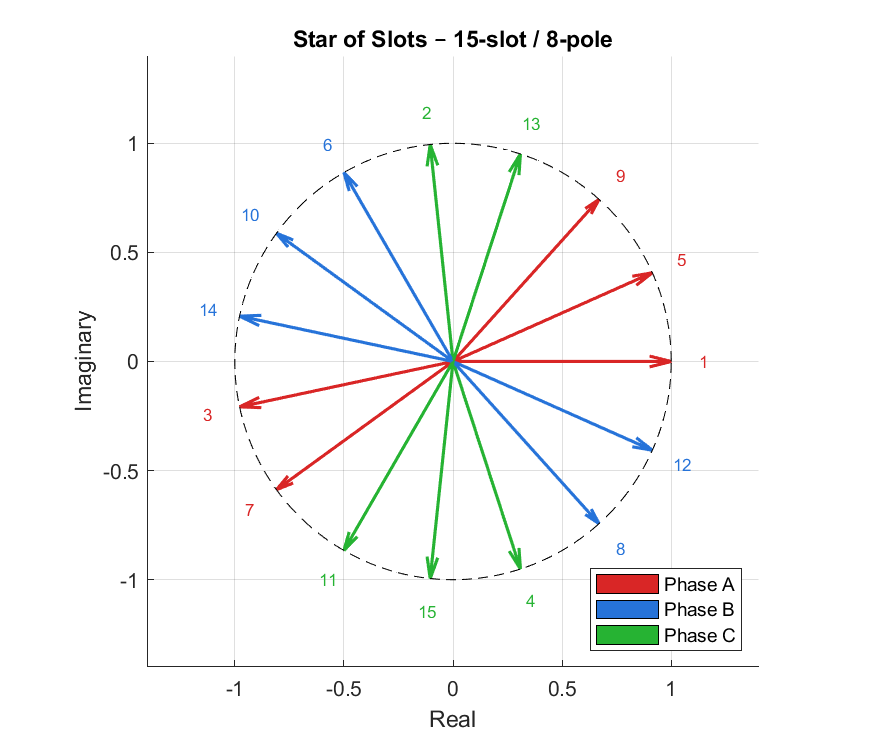
\includegraphics[width=0.58\textwidth]{../q2_star_of_slots.png}
  \caption{Star of slots for Design~1 ($N_s=15$, $N_m=8$).
           Colours: red = Phase~A, blue = Phase~B, green = Phase~C.
           Solid arrows = positive direction; dashed = negative direction.}
  \label{fig:q2_star}
\end{figure}

% ---- 2.4 -------------------------------------------------------
\subsection{Step 4 -- Winding Factor by Phasor Summation}

\subsubsection{Calculation Method}

For the $n$-th space harmonic, each slot assigned to Phase~A contributes one
unit phasor.
The angle of that phasor depends on whether the slot is positive or negative
(Eq.~\eqref{eq:kw_fscw}):
\begin{equation}
  \text{A$+$ slot $k$:} \quad e^{\,j\,n\,\varphi_k},
  \qquad
  \text{A$-$ slot $k$:} \quad e^{\,j\,(n\,\varphi_k\;+\;180\degree)}
  \label{eq:phasor_contrib}
\end{equation}
The winding factor is then the magnitude of the vector sum divided by the
number of slots per phase ($N_{ph} = 5$):
\begin{equation}
  k_{w,n} = \frac{\bigl|\Sigma_A\bigr|}{N_{ph}} = \frac{\bigl|\Sigma_A\bigr|}{5}
\end{equation}
The A$-$ slots effectively have their phasors \emph{reversed} (rotated
$180\degree$) before summing, which accounts for the fact that the
current flows in the opposite direction in those slots.

\subsubsection{Fundamental ($n = 1$)}

\begin{table}[H]
  \centering\small
  \caption{Phase~A phasor contributions, $n=1$}
  \label{tab:q2_ph1}
  \begin{tabular}{cccccc}
    \toprule
    Slot & Type & $\varphi_k$ & Angle used ($n\varphi_k$+rev.) & Real & Imag. \\
    \midrule
    1 & A$+$ & $  0\degree$ & $  0\degree$          & $+1.000$ & $+0.000$ \\
    5 & A$+$ & $ 24\degree$ & $ 24\degree$          & $+0.914$ & $+0.407$ \\
    9 & A$+$ & $ 48\degree$ & $ 48\degree$          & $+0.669$ & $+0.743$ \\
    3 & A$-$ & $192\degree$ & $192\degree+180\degree=12\degree$ & $+0.978$ & $+0.208$ \\
    7 & A$-$ & $216\degree$ & $216\degree+180\degree=36\degree$ & $+0.809$ & $+0.588$ \\
    \midrule
    \multicolumn{4}{r}{\textbf{Sum $\Sigma_A$}} & $+4.370$ & $+1.946$ \\
    \bottomrule
  \end{tabular}
\end{table}
\begin{equation}
  |\Sigma_A| = \sqrt{4.370^2 + 1.946^2} = \sqrt{19.10 + 3.79} = 4.783
\end{equation}
\begin{equation}
  \boxed{k_{w,1} = \frac{4.783}{5} = 0.9566}
\end{equation}

\noindent\textbf{Observation:} After reversing the A$-$ phasors (slots~3 and~7),
all five phasors cluster in the first quadrant within a $48\degree$ arc.
They nearly align, which explains the high winding factor.

\subsubsection{Third Harmonic ($n = 3$)}

For $n=3$ the phasor angle of each slot is multiplied by~3 before applying
the reversal for A$-$ slots.

\begin{table}[H]
  \centering\small
  \caption{Phase~A phasor contributions, $n=3$}
  \label{tab:q2_ph3}
  \begin{tabular}{cccccc}
    \toprule
    Slot & Type & $\varphi_k$ & Angle used ($3\varphi_k$+rev.) & Real & Imag. \\
    \midrule
    1 & A$+$ & $  0\degree$ & $  0\degree$                    & $+1.000$ & $+0.000$ \\
    5 & A$+$ & $ 24\degree$ & $ 72\degree$                    & $+0.309$ & $+0.951$ \\
    9 & A$+$ & $ 48\degree$ & $144\degree$                    & $-0.809$ & $+0.588$ \\
    3 & A$-$ & $192\degree$ & $576\degree+180\degree=36\degree$ & $+0.809$ & $+0.588$ \\
    7 & A$-$ & $216\degree$ & $648\degree+180\degree=108\degree$ & $-0.309$ & $+0.951$ \\
    \midrule
    \multicolumn{4}{r}{\textbf{Sum $\Sigma_A$}} & $+1.000$ & $+3.078$ \\
    \bottomrule
  \end{tabular}
\end{table}
\begin{equation}
  |\Sigma_A| = \sqrt{1.000^2 + 3.078^2} = \sqrt{1.000 + 9.474} = 3.236
\end{equation}
\begin{equation}
  \boxed{k_{w,3} = \frac{3.236}{5} = 0.6472}
\end{equation}

\subsubsection{Fifth Harmonic ($n = 5$)}

\begin{table}[H]
  \centering\small
  \caption{Phase~A phasor contributions, $n=5$}
  \label{tab:q2_ph5}
  \begin{tabular}{cccccc}
    \toprule
    Slot & Type & $\varphi_k$ & Angle used ($5\varphi_k$+rev.) & Real & Imag. \\
    \midrule
    1 & A$+$ & $  0\degree$ & $   0\degree$                     & $+1.000$ & $+0.000$ \\
    5 & A$+$ & $ 24\degree$ & $ 120\degree$                     & $-0.500$ & $+0.866$ \\
    9 & A$+$ & $ 48\degree$ & $ 240\degree$                     & $-0.500$ & $-0.866$ \\
    3 & A$-$ & $192\degree$ & $960\degree+180\degree=60\degree$  & $+0.500$ & $+0.866$ \\
    7 & A$-$ & $216\degree$ & $1080\degree+180\degree=180\degree$& $-1.000$ & $+0.000$ \\
    \midrule
    \multicolumn{4}{r}{\textbf{Sum $\Sigma_A$}} & $-0.500$ & $+0.866$ \\
    \bottomrule
  \end{tabular}
\end{table}
\begin{equation}
  |\Sigma_A| = \sqrt{(-0.500)^2 + (0.866)^2} = \sqrt{0.250 + 0.750} = 1.000
\end{equation}
\begin{equation}
  \boxed{k_{w,5} = \frac{1.000}{5} = 0.200}
\end{equation}

\noindent\textbf{Observation:} The three A$+$ slots lie at $0\degree$,
$120\degree$, $240\degree$ -- a balanced triphasic set whose vector sum is
exactly zero.
The A$-$ slots only partially restore the sum, resulting in a very small
$|\Sigma_A| = 1.0$, hence the low $k_{w,5}$.

\begin{table}[H]
  \centering
  \caption{Summary of winding factors -- Design~1 (15-slot/8-pole)}
  \label{tab:q2_kw}
  \begin{tabular}{lcccc}
    \toprule
    Harmonic & $\Sigma_A$ & $|\Sigma_A|$ & $k_{w,n}$ & Note \\
    \midrule
    $n=1$ (fund.) & $4.370+j1.946$ & 4.783 & \textbf{0.9566} & High; good torque density \\
    $n=3$ (triplen) & $1.000+j3.078$ & 3.236 & 0.6472 & Zero-seq.; no net torque \\
    $n=5$ & $-0.500+j0.866$ & 1.000 & 0.2000 & Naturally suppressed \\
    \bottomrule
  \end{tabular}
\end{table}

Figure~\ref{fig:q2_phasors} shows the Phase~A phasor diagrams for all three
harmonics.
Each arrow is one slot phasor (after reversing A$-$ slots);
the thick red arrow is the vector resultant.

\begin{figure}[H]
  \centering
  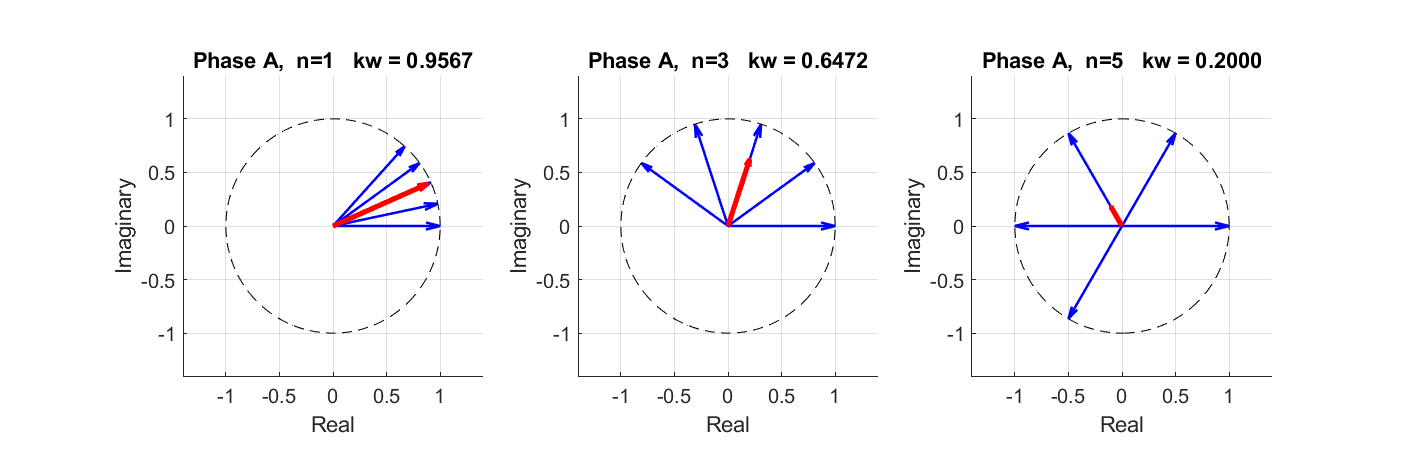
\includegraphics[width=\textwidth]{../q2_phase_A_phasors.png}
  \caption{Phase~A phasor diagrams for $n=1,3,5$.
           Blue arrows = individual slot phasors; red arrow = vector sum.
           Winding factor $= |\text{sum}|/5$.}
  \label{fig:q2_phasors}
\end{figure}

% ---- Note on the concentrated-coil convention -----------------
\subsubsection*{Note on the Concentrated-Coil Convention}

The phasor sum above uses only the five \emph{go-side} positions of Phase~A
(Layer~1: slots 1, 5, 9, 3, 7).
The return-sides (Layer~2) of these coils are \emph{not} added as extra phasors --
and this is intentional.

In a fractional-slot \textbf{concentrated} (single-tooth) winding each coil is
wound around \emph{one} tooth.
Following the convention used by Hanselman \cite{Hanselman2006}, each coil is
represented by a \emph{single phasor placed at its tooth-centre angle}, and the
winding factor is the vector sum of the five coil phasors divided by~5:
\begin{equation}
  k_{w,n} \;=\; \frac{\bigl|\sum_{i=1}^{5} e^{\,j\,n\,\varphi_i}\bigr|}{5}
  \quad\text{(coil phasors at tooth centres).}
  \label{eq:kw_concentrated}
\end{equation}
The return-side is the same physical conductor as the go-side -- both
together form a single coil -- so adding it as a second phasor would be
double counting.
For the design equations used in this report
(EMF, torque, shear stress, turns/phase, $\,\S\,\ref{sec:q3}$) the correct
quantity is the concentrated-coil value $k_{w,1} = 0.9566$.

% ---- 2.5 -------------------------------------------------------
\subsection{Step 5 -- Constructing the Winding Diagram}

\subsubsection{From Slot Assignments to Physical Coils}

The star-of-slots gave us \emph{one assignment per slot} -- the \emph{upper
(Layer~1)} of each slot.
In the physical machine each slot has \textbf{two} coil-side layers, and
each coil is wound around \textbf{one tooth} (concentrated / tooth-coil winding).

\noindent The double-layer layout follows two rules:
\begin{enumerate}
  \item \textbf{Layer~1 of slot $k$} $=$ star-of-slots assignment
        (Table~\ref{tab:q2_assignment}) -- the \emph{go-side} of the coil
        on tooth $k$.
  \item \textbf{Layer~2 of slot $k$} $=$ \emph{opposite} of Layer~1 of slot
        $k-1$ (circular: slot~0 $\equiv$ slot~15):
        \begin{equation}
          \text{Layer-2}[k] = -\,\text{Layer-1}[k-1]
          \label{eq:q2_lower}
        \end{equation}
        This is the \emph{return-side} of the coil on tooth $k-1$.
\end{enumerate}

\noindent\textbf{Physical meaning of Eq.~\eqref{eq:q2_lower}:}
Tooth $k-1$ sits between slot $k-1$ and slot $k$.
A coil wound around tooth $k-1$ has its go-side in Layer~1 of slot $k-1$
and its return-side in Layer~2 of slot $k$.
The return side always carries the \emph{opposite} current direction.

\begin{center}
\begin{tabular}{ccccc}
  Slot $k-1$ & & Tooth $k-1$ & & Slot $k$ \\
  \framebox[2.5cm]{Layer~1: Phase~X$+$} &
  $\xrightarrow{\;\text{coil}\;}$ & & $\xrightarrow{}$ &
  \framebox[2.5cm]{Layer~2: Phase~X$-$} \\
  go-side & & & & return-side \\
\end{tabular}
\end{center}

\subsubsection{Worked Example (Slot 4)}

Layer-1[4] $=$ C$+$ (from Table~\ref{tab:q2_assignment}).\\
Layer-2[4] $= -$Layer-1[3] $= -$(A$-$) $=$ A$+$.\\
This means slot~4 has C$+$ in the upper layer and A$+$ in the lower layer.
These belong to \emph{different} phases -- a normal feature of double-layer FSCWs.

\subsubsection{Coil Identification Table}

Table~\ref{tab:q2_coils} shows all 15 coils (one per tooth).
The go-side is always Layer~1 of slot $k$; the return-side is always
Layer~2 of slot $k+1$ (which is the opposite of Layer~1 of slot $k$,
confirming every coil is single-phase).

\begin{table}[H]
  \centering\small
  \caption{Coil table -- 15 tooth-wound coils}
  \label{tab:q2_coils}
  \begin{tabular}{cclcc}
    \toprule
    Tooth & Go-side: Layer-1[slot $k$] & Return-side: Layer-2[slot $k{+}1$] & Phase \\
    \midrule
     1 & Slot\;1: A$+$ & Slot\;2: A$-$  & A \\
     2 & Slot\;2: C$-$ & Slot\;3: C$+$  & C \\
     3 & Slot\;3: A$-$ & Slot\;4: A$+$  & A \\
     4 & Slot\;4: C$+$ & Slot\;5: C$-$  & C \\
     5 & Slot\;5: A$+$ & Slot\;6: A$-$  & A \\
     6 & Slot\;6: B$+$ & Slot\;7: B$-$  & B \\
     7 & Slot\;7: A$-$ & Slot\;8: A$+$  & A \\
     8 & Slot\;8: B$-$ & Slot\;9: B$+$  & B \\
     9 & Slot\;9: A$+$ & Slot\;10: A$-$ & A \\
    10 & Slot\;10: B$+$ & Slot\;11: B$-$ & B \\
    11 & Slot\;11: C$+$ & Slot\;12: C$-$ & C \\
    12 & Slot\;12: B$-$ & Slot\;13: B$+$ & B \\
    13 & Slot\;13: C$-$ & Slot\;14: C$+$ & C \\
    14 & Slot\;14: B$+$ & Slot\;15: B$-$ & B \\
    15 & Slot\;15: C$+$ & Slot\;1:\;C$-$ & C \\
    \bottomrule
  \end{tabular}
\end{table}

\noindent Coil distribution:
\textbf{Phase A} -- teeth 1, 3, 5, 7, 9;\quad
\textbf{Phase B} -- teeth 6, 8, 10, 12, 14;\quad
\textbf{Phase C} -- teeth 2, 4, 11, 13, 15.

\noindent Note the grouping pattern: Phase~A occupies five consecutive odd-numbered
teeth (1--9), Phase~B five alternating teeth in the upper half (6--14),
and Phase~C the remaining five teeth.
This non-uniform spacing (unlike the regular ABC pattern of integral-slot
windings) is a direct consequence of the fractional-slot geometry.

\subsubsection{Double-Layer Slot Table}

Combining Layer~1 (from Table~\ref{tab:q2_assignment}) and Layer~2
(from Eq.~\eqref{eq:q2_lower}) gives the full double-layer layout:

\begin{table}[H]
  \centering\small
  \caption{Double-layer slot layout -- Design~1 (15-slot/8-pole)}
  \label{tab:q2_doublelayer}
  \begin{tabular}{c|cc||c|cc}
    \toprule
    Slot & Layer~1 (Upper) & Layer~2 (Lower) &
    Slot & Layer~1 (Upper) & Layer~2 (Lower) \\
    \midrule
     1 & A$+$ & C$-$ &  9 & A$+$ & B$+$ \\
     2 & C$-$ & A$-$ & 10 & B$+$ & A$-$ \\
     3 & A$-$ & C$+$ & 11 & C$+$ & B$-$ \\
     4 & C$+$ & A$+$ & 12 & B$-$ & C$-$ \\
     5 & A$+$ & C$-$ & 13 & C$-$ & B$+$ \\
     6 & B$+$ & A$-$ & 14 & B$+$ & C$+$ \\
     7 & A$-$ & B$-$ & 15 & C$+$ & B$-$ \\
     8 & B$-$ & A$+$ &    &      &      \\
    \bottomrule
  \end{tabular}
\end{table}

\noindent\textbf{How to read the table:}
Each row is one slot.
Layer~1 (upper, closer to the air gap) is always the go-side of one coil.
Layer~2 (lower) is always the return-side of the adjacent coil (on the
preceding tooth).
In most slots two \emph{different} phases share the same slot
(e.g., slot~1 has A$+$ above and C$-$ below) -- this is entirely normal
for a double-layer FSCW.

The full winding layout is shown in Figure~\ref{fig:q2_winding}.
Each arc in the figure represents one tooth-wound coil connecting the two
adjacent slots of that tooth.

\begin{figure}[H]
  \centering
  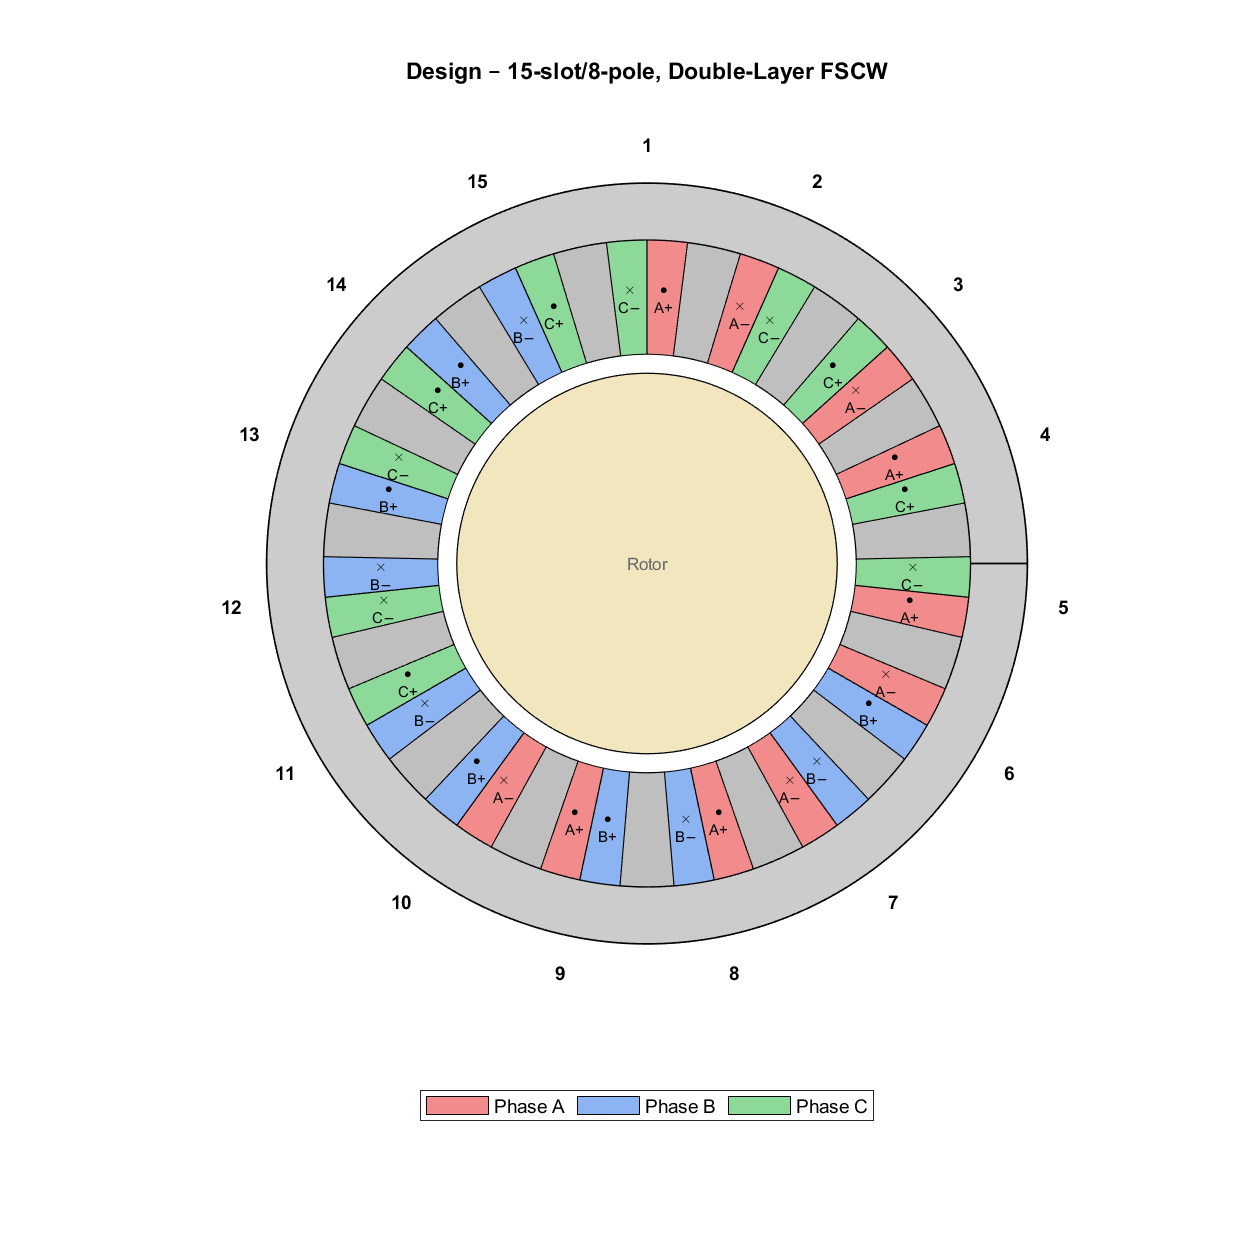
\includegraphics[width=0.65\textwidth]{../q2_winding_layout.png}
  \caption{Winding layout for Design~1 (15-slot/8-pole, 3-phase).
           Each arc = one tooth-wound coil.
           Red = Phase A (teeth 1,3,5,7,9),
           blue = Phase B (teeth 6,8,10,12,14),
           green = Phase C (teeth 2,4,11,13,15).
           $\bullet$ = current into page; $\times$ = current out of page.}
  \label{fig:q2_winding}
\end{figure}

% ---- 2.6 -------------------------------------------------------
\subsection{Step 6 -- Verification: Valid and Balanced Winding}

A winding is \emph{valid} if every slot is occupied and every coil belongs
to exactly one phase.
A winding is \emph{balanced} if all three phases produce equal RMS EMFs
displaced by $120\degree$.

\begin{enumerate}

\item \textbf{All slots occupied.}
  Table~\ref{tab:q2_doublelayer} fills all $15 \times 2 = 30$ conductor
  positions with no gaps.

\item \textbf{Every coil is single-phase.}
  Table~\ref{tab:q2_coils} shows that the go-side and return-side of every
  coil carry the same phase letter (only the $\pm$ sign differs, as required
  for a coil).
  No coil mixes phases.

\item \textbf{Equal conductors per phase.}
  Each phase has 5 coils $= 10$ conductor positions out of 30 total
  ($= 1/3$) -- identical for A, B, and C.

\item \textbf{Balanced phase resultants.}
  By the three-fold symmetry of the winding ($\gcd(15,3)=3$),
  the phasor resultants of phases B and C have the same magnitude as
  Phase~A ($|\Sigma_B| = |\Sigma_C| = 4.783$ for $n=1$) and are displaced
  by exactly $120\degree$.

\item \textbf{Winding factor check.}
  $k_{w,1} = 0.9566$ is consistent with the value tabulated in
  \cite[Table~]{Hanselman2006} for the 15/8 slot-pole combination,
  confirming the phasor summation is correct.

\end{enumerate}

% ---- 2.7 -------------------------------------------------------
\subsection{Discussion}

\begin{enumerate}

\item \textbf{High fundamental winding factor for a concentrated winding.}
  $k_{w,1} = 0.9566$ is comparable to that of distributed windings
  (typically 0.925--0.966) and far above the minimum ($\approx 0.5$) for
  random concentrated windings.
  The 15/8 combination is specifically identified in \cite{Hanselman2006}
  as one of the best fractional-slot combinations for torque density.

\item \textbf{Natural suppression of the 5th harmonic.}
  The three A$+$ slots contribute phasors at $0\degree$, $120\degree$,
  $240\degree$ for $n=5$ -- a balanced triphasic set that sums to zero.
  Only the A$-$ slots restore a small residual ($|\Sigma|=1.0$),
  giving $k_{w,5} = 0.2$.
  This suppression is geometric and requires no pitch adjustment.

\item \textbf{3rd harmonic: large winding factor, zero net rotating field.}
  $k_{w,3} = 0.647$ is large, but as discussed in Q1, the 3rd space
  harmonic is triplen: all three phases produce it in the same spatial
  direction, and the balanced condition $I_A + I_B + I_C = 0$ cancels the
  net rotating component.
  It may still cause iron losses through standing-wave effects.

\item \textbf{Two phases share each slot.}
  Unlike integral-slot windings where each slot is occupied by a single
  phase, the double-layer FSCW places two \emph{different} phases in each
  slot.
  This is unavoidable when $q < 1$: adjacent teeth belong to different
  phases, and each slot borders two adjacent teeth.

\item \textbf{Short end-windings -- key FSCW advantage.}
  Because each coil spans only one tooth pitch (approximately
  $360\degree/(N_s) = 24\degree$ mechanical), the overhang is very short.
  This reduces copper volume, DC resistance, and copper losses -- the
  primary advantage of FSCWs for direct-drive, high-torque-density
  applications \cite{Meier2008}.

\end{enumerate}

% ============================================================
\section{Q3 -- Analytical Modelling}
\label{sec:q3}

\subsection{Machine Dimensions}

From the assignment common specifications and the Design~1 ratio
$R_{ro}/R_{so} = 0.6$:

\begin{table}[H]
  \centering
  \caption{Machine geometry -- Design~1}
  \label{tab:q3_geometry}
  \begin{tabular}{lll}
    \toprule
    Parameter & Symbol & Value \\
    \midrule
    Stator outer radius          & $R_{so}$           & 50.0\unit{mm} \\
    Rotor outer radius           & $R_{ro}=0.6\,R_{so}$ & 30.0\unit{mm} \\
    Air-gap length               & $g$                & 1.0\unit{mm}  \\
    Magnet radial thickness      & $l_m$              & 4.0\unit{mm}  \\
    Stator inner radius          & $R_{si}=R_{ro}+g$  & 31.0\unit{mm} \\
    Rotor core outer radius      & $R_{ro,c}=R_{ro}-l_m$ & 26.0\unit{mm} \\
    Stack length                 & $L_s$              & 100\unit{mm}  \\
    Magnet remanence             & $B_r$              & 1.3\unit{T}   \\
    Magnet relative permeability & $\mu_r$            & 1.05          \\
    Magnet arc ratio             & $\alpha_m$         & 0.889         \\
    Target iron flux density     & $B_t$              & 1.4\unit{T}   \\
    Current density (rms)        & $J_{rms}$          & 5\unit{A/mm^2}\\
    Slot fill factor             & $k_{wc}$           & 0.60          \\
    \bottomrule
  \end{tabular}
\end{table}

\subsection{Slot Pitch and Tooth Geometry}

The slot pitch at the stator bore:
\begin{equation}
  \tau_s = \frac{2\pi R_{si}}{N_s}
         = \frac{2\pi \times 31}{15} = 12.99\unit{mm}
\end{equation}

A first-pass estimate of the peak air-gap flux density without Carter
correction gives $B_{g,0} = B_r l_m/(l_m + \mu_r g) = 1.030\unit{T}$.
The average flux density under the magnet arc is
$B_{g,\text{avg}} = B_{g,0}\,\alpha_m = 1.030 \times 0.889 = 0.916\unit{T}$.
For $B_t = 1.4\unit{T}$ in the teeth:
\begin{equation}
  w_{tb} = \frac{B_{g,\text{avg}}\,\tau_s}{B_t}
         = \frac{0.916 \times 12.99}{1.4} = 8.50\unit{mm}
\end{equation}
\begin{equation}
  w_s = \tau_s - w_{tb} = 12.99 - 8.50 = 4.49\unit{mm}
\end{equation}

\subsection{Carter's Coefficient}

Applying Eq.~\eqref{eq:kc} with $g = 1\unit{mm}$ and $w_s = 4.49\unit{mm}$:
\begin{equation}
  x = \frac{w_s}{2g} = \frac{4.49}{2} = 2.245
\end{equation}
\begin{equation}
  \gamma = \frac{4 \times 1}{\pi}\bigl[2.245\arctan(2.245)
           - \ln\!\sqrt{1+2.245^2}\bigr]
         = \frac{4}{\pi}\bigl[2.245\times1.150 - 0.899\bigr]
         = 2.143\unit{mm}
\end{equation}
\begin{equation}
  k_c = \frac{12.99}{12.99 - 2.143} = \mathbf{1.197}
\end{equation}

\subsection{Effective Air Gap and Corrected Flux Density}

\begin{equation}
  g_{\text{eff}} = k_c\,g + \frac{l_m}{\mu_r}
                 = 1.197 \times 1 + \frac{4}{1.05}
                 = 1.197 + 3.810 = 5.007\unit{mm}
\end{equation}

Substituting into Eq.~\eqref{eq:Bg}:
\begin{equation}
  B_{g,\text{peak}} = \frac{1.3 \times 4}{4 + 1.05 \times 1.197 \times 1}
                    = \frac{5.2}{5.257} = \mathbf{0.989\unit{T}}
\end{equation}

\subsection{Effective Axial Length}

From Eq.~\eqref{eq:Le}:
\begin{equation}
  L_e = 100 + 2 \times 1 = \mathbf{102\unit{mm}}
\end{equation}

\subsection{Air-Gap Peak Flux Density Summary}

All three values are consistent: the slotting correction reduces
$B_{g,\text{peak}}$ from 1.030\unit{T} (idealised) to 0.989\unit{T}
(with Carter correction), a reduction of 3.9\%.

\subsection{Flux Per Pole}

From Eq.~\eqref{eq:Phi}:
\begin{equation}
  \tau_p = \frac{\pi \times 31}{4} = 24.35\unit{mm}
\end{equation}
\begin{equation}
  \Phi_{pole} = 0.989 \times 0.889 \times 24.35\times10^{-3}
                \times 102\times10^{-3}
              = \mathbf{2.18\unit{mWb}}
\end{equation}

\subsection{Magnetic Loading}

\begin{equation}
  \bar{B} = B_{g,\text{peak}} \cdot \alpha_m = 0.989 \times 0.889
          = \mathbf{0.879\unit{T}}
\end{equation}

\subsection{Iron Yoke Widths}

From Eq.~\eqref{eq:yoke}:
\begin{equation}
  w_{sy} = w_{ry} = \frac{2.18\times10^{-3}}{2 \times 1.4 \times 0.102}
         = \mathbf{7.64\unit{mm}}
\end{equation}
The rotor shaft radius is
$R_{ro,c} - w_{ry} = 26 - 7.64 = 18.4\unit{mm}$.

\subsection{Electrical Loading}

Available slot height and slot area (rectangular approximation):
\begin{equation}
  h_{slot} = (R_{so} - R_{si}) - w_{sy} = 19 - 7.64 = 11.36\unit{mm}
\end{equation}
\begin{equation}
  A_{slot} = w_s \times h_{slot} = 4.49 \times 11.36 = 51.0\unit{mm^2}
\end{equation}

From Eq.~\eqref{eq:Arms}:
\begin{equation}
  A_{rms} = \frac{5 \times 0.60 \times 51.0}{12.99} = \mathbf{11.78\unit{kA/m}}
\end{equation}

\subsection{Shear Stress and Expected Torque}

From Eqs.~\eqref{eq:sigma}--\eqref{eq:T}:
\begin{equation}
  \sigma = \frac{1}{\sqrt{2}} \times 0.9566 \times 0.989 \times 11{,}780
         = \mathbf{7.87\unit{kPa}}
\end{equation}
\begin{equation}
  T = 7870 \times 2\pi \times (0.031)^2 \times 0.102
    = \mathbf{4.85\unit{N \cdot m}}
\end{equation}
\begin{equation}
  P = 4.85 \times \frac{1500 \times 2\pi}{60} = \mathbf{762\unit{W}}
\end{equation}

The shear stress of 7.87\unit{kPa} is consistent with the range
5--35\unit{kPa} quoted for liquid-cooled PMSMs in
\cite[Ch.\,3]{Hanselman2006}.

\subsection{Number of Turns Per Phase}

For $V_{dc} = 48\unit{V}$ (star connection), the peak phase voltage is:
\begin{equation}
  \hat{V}_{ph} = \frac{V_{dc}}{\sqrt{3}} = \frac{48}{\sqrt{3}} = 27.7\unit{V}
\end{equation}
The electrical angular frequency at $n = 1500\unit{rpm}$:
\begin{equation}
  \omega_e = p\,\omega_m = 4 \times \frac{1500 \times 2\pi}{60}
           = 628.3\unit{rad/s}
\end{equation}
The required number of turns per phase \cite[Ch.\,2]{Hanselman2006}:
\begin{equation}
  N_{ph} = \frac{\hat{V}_{ph}}{k_{w,1}\,\omega_e\,\Phi_{pole}}
         = \frac{27.7}{0.9566 \times 628.3 \times 2.18\times10^{-3}}
         \approx 21.2
\end{equation}
Rounding to an integer number of conductors per slot
($N_{cs} = 2N_{ph}m/N_s$, must be integer):
\begin{equation}
  N_{cs} = 8 \implies N_{ph} = \frac{8 \times 15}{2 \times 3} = 20
\end{equation}
Back-EMF at 1500\unit{rpm}:
$\hat{E}_{ph} = 0.9566 \times 628.3 \times 2.18\times10^{-3} \times 20
             = 26.2\unit{V}$

\subsection{Summary of Analytical Results}

\begin{table}[H]
  \centering
  \caption{Analytical modelling results -- Design~1}
  \label{tab:q3_summary}
  \begin{tabular}{lll}
    \toprule
    Parameter & Symbol & Value \\
    \midrule
    Slot pitch              & $\tau_s$           & 12.99\unit{mm} \\
    Tooth width             & $w_{tb}$           & 8.50\unit{mm}  \\
    Slot opening            & $w_s$              & 4.49\unit{mm}  \\
    Carter coefficient      & $k_c$              & 1.197 \\
    Effective air gap       & $g_{\text{eff}}$   & 5.007\unit{mm} \\
    Effective axial length  & $L_e$              & 102\unit{mm}   \\
    Air-gap peak flux density & $B_{g,\text{peak}}$ & 0.989\unit{T} \\
    Flux per pole           & $\Phi_{pole}$      & 2.18\unit{mWb} \\
    Magnetic loading        & $\bar{B}$          & 0.879\unit{T}  \\
    Stator yoke width       & $w_{sy}$           & 7.64\unit{mm}  \\
    Rotor yoke width        & $w_{ry}$           & 7.64\unit{mm}  \\
    Slot height             & $h_{slot}$         & 11.36\unit{mm} \\
    Electrical loading (rms)& $A_{rms}$          & 11.78\unit{kA/m} \\
    Shear stress            & $\sigma$           & 7.87\unit{kPa} \\
    Expected torque         & $T$                & 4.85\unit{N{\cdot}m} \\
    Expected output power   & $P$                & 762\unit{W}    \\
    Turns per phase         & $N_{ph}$           & 20             \\
    Conductors per slot     & $N_{cs}$           & 8              \\
    \bottomrule
  \end{tabular}
\end{table}

% ============================================================
\section{Q4 -- 2D FEA Modelling (ANSYS Maxwell)}
\label{sec:q4}

\textit{(To be completed after ANSYS Maxwell simulation.)}

The following results will be obtained from the 2D magnetostatic/transient
simulation in ANSYS Maxwell:

\begin{enumerate}[noitemsep]
  \item Flux density distribution in the stator core, with maximum values
        verified against $B_t = 1.4\unit{T}$ in teeth and back-iron.
  \item Air-gap flux density at the mid-gap radius plotted vs.\
        circumferential angle.
  \item Leakage flux path visualisation (slot leakage, magnet-to-magnet,
        tip leakage, magnet--tooth--magnet).
  \item Flux per pole from FEA (to be compared with
        $\Phi_{pole}^{\text{analytical}} = 2.18\unit{mWb}$).
  \item (Bonus) Cogging torque vs.\ rotor angle.
\end{enumerate}

% ============================================================
\section*{References}
\addcontentsline{toc}{section}{References}

\begin{thebibliography}{9}

\bibitem{Pyrhonen2014}
J.~Pyrh\"onen, T.~Jokinen, and V.~Hrabovcov{\'a},
\textit{Design of Rotating Electrical Machines}, 2nd ed.
Chichester, UK: Wiley, 2014.

\bibitem{Hanselman2006}
D.~C.~Hanselman,
\textit{Brushless Permanent Magnet Motor Design}, 2nd ed.
Lebanon, NH: Magna Physics, 2006.

\bibitem{Chapman2012}
S.~J.~Chapman,
\textit{Electric Machinery Fundamentals}, 5th ed.
New York: McGraw-Hill, 2012.

\bibitem{Meier2008}
F.~Meier,
``Permanent-magnet synchronous machines with non-overlapping concentrated
windings for low-speed direct-drive applications,''
Ph.D.\ dissertation, Royal Institute of Technology (KTH), Stockholm,
Sweden, 2008.
[Online]. Available: \url{http://www.diva-portal.org/smash/get/diva2:332/FULLTEXT01.pdf}

\bibitem{Carter1901}
F.~W.~Carter,
``Air-gap induction,''
\textit{Electrical World and Engineer}, vol.~38, pp.~884--888, 1901.

\bibitem{HW2Def}
EE568 Course Staff,
``EE568 Project-2: Motor Winding Design \& Analysis,'' METU, 2026.

\end{thebibliography}

% ============================================================
\appendix
\section{MATLAB Script}

The complete MATLAB script \texttt{ee568\_hw2\_analytical.m} is submitted
alongside this report. It computes all Q1--Q3 results, generates the winding diagrams and phasor
plots in Section~\ref{sec:q2} (Figures \ref{fig:q2_star}--\ref{fig:q2_winding}),
and prints a summary table to the console.

\end{document}
